\documentclass{classrep}
\usepackage[utf8]{inputenc}
\usepackage{color}
\usepackage{float}
\usepackage{graphicx}

\usepackage{amsmath}
\usepackage{booktabs}
\usepackage{listings}
\usepackage{multirow}
\usepackage{siunitx}
\usepackage{tabu}

\newcommand\foreign[1]{#1}
\newcommand\code[1]{\texttt{#1}}
\newcommand\underscore[0]{\char`_}

\lstset{
  language=Bash,
  basicstyle=\scriptsize\ttfamily,
  showspaces=false,
  showstringspaces=false,
  frame=single,
  frameround=tttt,
  breaklines=true,
  breakatwhitespace=false,
  extendedchars=true,
  inputencoding=utf8,
  literate={ą}{{\k{a}}}1 {ć}{{\'c}}1 {ę}{{\k{e}}}1 {ł}{{\l{}}}1 {ń}{{\'n}}1 {ó}{{\'o}}1 {ś}{{\'s}}1 {ż}{{\.z}}1 {ź}{{\'z}}1 {Ą}{{\k{A}}}1 {Ć}{{\'C}}1 {Ę}{{\k{E}}}1 {Ł}{{\L{}}}1 {Ń}{{\'N}}1 {Ó}{{\'O}}1 {Ś}{{\'S}}1 {Ż}{{\.Z}}1 {Ź}{{\'Z}}1 {‘}{`}1 {’}{'}1 {•}{{\textbullet}}1
}

\studycycle{Computer science, stationary program, graduate studies.}
\coursesemester{II}

\coursename{Security of Information Systems}
\courseyear{2016/2017}

\courseteacher{Ph.D. Eng. Rafał Grzybowski}
\coursegroup{Tuesday, 12:15}

\author{
  \studentinfo{Michał Sośnicki}{207597} \and
  \studentinfo{Daniel Pęczek}{207585}
}

\title{Secure file transfer - practical part}

\begin{document}
\maketitle
\newpage

\section{Purpose}

The aim of the workshop is to find and implement a solution to the problem of secure file transfer. 
The final solution is required to be user-friendly, to an extend where it would be possible to utilize 
it in an average business, by people with limited technical knowledge. This report describes how we
have solved the problem by securing the data transmission with Gnu Privacy Guard, which is widely
regarded as secure. The method of transmission that we use is e-mail, which is nowadays familiar to
most people. Both technologies work well with each other and are easy to use with a proper setup.

\section{Problem statement}

A transmission can be considered secure if it has three following properties: 

\begin{enumerate}
\item Confidentiality - a file sent cannot be read by anyone other than the intended recipient.
\item Integrity - a file cannot be modified, neither by error nor with malicious intent, without this fact becoming known to the recipient.
\item Nonrepudiation - it is possible to verify if the file has been sent by the stated sender or if someone is trying to impersonate them. On the other hand, the true sender cannot deny that they have sent the message. 
\end{enumerate}

File transfer in the presented solution is limited by the capabilities of e-mail servers. The servers
usually refuse to handle files over hundreds of megabytes in size and usually work with significant
delays. Those limits seem however perfectly acceptable for the purposes of businesses and office
workers and they are our target as stated in the previous section.

GNU Privacy Guard provides the security with the following mechanisms:

\begin{enumerate}
\item Encrypting the message with the recipient public key makes the message confidential, since only they
    will be able to decrypt it with their private key. Other people will be unable to read it even if they
    manage to obtain it.
\item Digital signatures, created by calculating a hash of the message and encrypting it with the sender's
    private key, guarantee integrity and nonrepudiation. Anyone can verify if the messages comes from
    the sender by decrypting the signature with the sender's public key. (safely distributing the public
    keys is a concern, but it is also handled by GPG) The decrypted hash is a proof that the message
    has not been tampered with, because it even though it's possible to find other messages with
    the same hash value, it is improbable that the other messages with equal hash will be valid 
    texts in the human language.
\end{enumerate}

\section{Implementation}

We implemented and tested our GPG setup on a system of several Docker containers. 
At first, we considered setting up virtual machines, but it was troublesome to provide
enough operational memory and Docker proved to be an economical and feasible alternative.

On listing \ref{lst:setup-docker-compose} there is a \code{docker-compose} file that starts five
docker containers. We run a separate container with a mail server, a key server container 
and three containers with PGP/Email users, called admin, Anna and Beata. Admin serves
a vital role in ensuring that users trust each other public keys, which we will describe later.

\begin{lstlisting}[label={lst:setup-docker-compose}, caption={Contents of docker-compose.yml file, orchestrating all containers.}]
version: '2'

services:
  mail-server:
    image: tvial/docker-mailserver:latest
    domainname: domain.com
    volumes:
      - ./config/:/tmp/docker-mailserver/
      - mail-server-data:/var/mail
  keyserver:
    build: ./keyserver
  key-admin:
    build: ./key-admin
    volumes:
      - mail-users-shared:/home/admin/shared/
  mail-user-anna:
    build: ./mail-user
    ports:
      - "42000:22"
    volumes:
      - ./setup-anna/:/home/user/setup/:ro
      - ./profile-anna/:/home/user/.thunderbird/
      - mail-users-shared:/home/user/shared/
  mail-user-beata:
    build: ./mail-user
    ports:
      - "42001:22"
    volumes:
      - ./setup-beata/:/home/user/setup/:ro
      - ./profile-beata/:/home/user/.thunderbird/
      - mail-users-shared:/home/user/shared/

volumes:
  mail-server-data:
    driver: local
  mail-users-shared:
    driver: local
\end{lstlisting}

\subsection{Server setup}

For e-mail server we use a container created from \code{docker-mailserver} image, which is
available for free use on Docker Hub. We configured the server by providing it a list of
accounts to create. At start the server will have accounts \code{anna@domain.com} and 
\code{beata@domain.com} for the two users that will try to communicate in our setup.

We set up the GPG keyserver by ourselves, a complete Dockerfile is shown on listing 
\ref{lst:setup-keyserver-dockerfile}. We simply install a sks 
(\foreign{synchronizing key server}) on a linux instance and change it's configuration
to ensure that it will not communicate with other keyservers, since we do not want
to send our fake keys to real keyservers. Then we ensure that the containers will
run the sks by default when started.

In real implementation of GPG to a business it would be perfectly fine to use public
keyservers and email servers, although free email servers often limit the size of
attachments and may be insufficient. This choice is however irrelevant for the security
of communication.

\begin{lstlisting}[label={lst:setup-keyserver-dockerfile}, caption={Dockerfile describing keyserver container.}]
FROM ubuntu:16.04

RUN apt-get update 

RUN apt-get install -y sks

RUN su debian-sks -c "/usr/sbin/sks build"
RUN echo "# Empty - Do not communicate with other keyservers." 
    >/etc/sks/mailsync
RUN echo "# Empty - Do not communicate with other keyservers." 
    >/etc/sks/membership
RUN echo "initstart=yes" > /etc/default/sks
RUN systemctl enable sks.service

EXPOSE 11371

CMD ["bash", "-c", "service sks start; sleep infinity"]
\end{lstlisting}

\subsection{User setup}

We now set up the mail and GPG on the client side. We use \code{thunderbird} mail client
and integrate it with GPG with \code{enigmail} plugin. The setup is simple, performed
in GUI and thus we will not show most of the configuration performed in GUI. On the other hand,
GPG setup is crucial and we presented it fully on listing \ref{lst:setup-user-init}.

The steps the user must perform are as follows:

\begin{enumerate}
\item Generate a private/public key pair for use by this user. The private key must not be shared
    or the transmission will no longer be secure, so it is crucial that the user is made aware of
    this fact.
\item Learn admin key id. We will describe who the admin is in the next section. The key id should
    preferably be transferred offline. For example admin that performs these steps on an user
    computer can carry it on a pendrive.
\item Download the full admin key from the keyserver using the key id.  We could also carry it on
    a pendrive but we decided to do this this way to detect any connection problems at this step.
\item After verifying that the downloaded key looks like the one that belongs to admin, sign the
    admin key with user's private key. This is a common procedure in GPG which signifies
    that the user has verified that the key really belongs to admin and can be trusted.
\item Mark the admin key as fully trusted. This will cause us to consider all keys signed
    by admin as valid and admin signed all and only keys belonging to the employees 
    in the business.
\item Send our keyid to admin so that they can download our key, sign it with their private key
    and thus mark is as valid. Since all users fully trust the admin, they will automatically
    consider our key valid. 
\end{enumerate}

Those steps will add us to so-called GPG Web of Trust.

\begin{lstlisting}[label={lst:setup-user-init}, caption={Script run by user.}]
# Create key
gpg2 --gen-key --batch /home/user/setup/gpg-params.txt
GPGKEY=$(gpg2 --list-keys --fingerprint | head -n4 | tail -n1 
        | tr -d ' ' | sed 's/^Keyfingerprint=//')

# Wait for admin to initialize
echo "Waiting for admin"
while [ ! -f /home/user/shared/admin-keyid.txt ]
do
  sleep 1
done

# Trust the admin
ADMIN_KEYID=$(cat /home/user/shared/admin-keyid.txt)
gpg2 --recv-keys $ADMIN_KEYID
echo "password" | gpg2 --batch --passphrase-fd 0 --pinentry-mode loopback 
    --quick-sign-key "$ADMIN_KEYID"
gpg2 --send-keys $ADMIN_KEYID
echo "$ADMIN_KEYID:4:" | gpg2 --import-ownertrust

# Share your key with the admin to get it signed
gpg2 --send-keys $GPGKEY
touch "/home/user/shared/user-keys/$GPGKEY"
\end{lstlisting}

The docker container created on listing \ref{lst:setup-user-dockerfile} install GPG and mentioned
email client. We then start a ssh server on the container, which will allow us to eventually 
run the \code{thunderbird}. Most of the steps here are however related to the use of \code{docker}
and not really important for the matter of securing file transmission.

\begin{lstlisting}[label={lst:setup-user-dockerfile}, caption={Dockerfile describing user container.}]
FROM ubuntu:16.04

RUN apt-get update 

# SSH server to run thunderbird remotely with X forwarding
RUN apt-get install -y openssh-server
RUN mkdir /var/run/sshd
EXPOSE 22

# Create user
RUN useradd -m "user"
RUN echo "user:password" | chpasswd

# Setup GPG
RUN apt-get install -y gnupg2 thunderbird enigmail
COPY gpg.conf /home/user/.gnupg/gpg.conf
COPY gpg-agent.conf /home/user/.gnupg/gpg-agent.conf
COPY init-gpg.sh /home/user/init-gpg.sh
RUN chown user:user /home/user/.gnupg /home/user/.gnupg/gpg.conf 
    /home/user/.gnupg/gpg-agent.conf /home/user/init-gpg.sh
RUN chmod +x /home/user/init-gpg.sh

RUN mkdir /home/user/shared
RUN chown user:user /home/user/shared

CMD ["bash", "-c", "su - user -c /home/user/init-gpg.sh; /usr/sbin/sshd -D"]
\end{lstlisting}

\subsection{Admin setup}

Key server and mail server are not enough for our setup to work. 
Users may send files between each other and have their own key pairs, but
they have no reason to trust each other keys. Some other person could
generate a key, send it to the key server and claim to be one of the employees.
To solve this problem, it is necessary to establish a Web of Trust between the users.

One way to do this would be to make sure a new employee takes their public key
to other employees in the business and makes them sign it. After several people
do this, other employees will eventually also consider it valid. This solution
has an advantage of being decentralized and is how the GPG is supposed to work
globally. In the company, however, we can centralize the process to make it 
faster and simpler.

The way we accomplish it is by creating an admin key pair. Each new employee
has its key signed by admin and then import, sign and mark the admin key pair as fully
trusted. Full trust means that they will automatically consider all keys
signed by admin as valid. In this way we can completely integrate a new person
in the company Web of Trust with only two import-sign steps.

Script run by the admin is shown on listing \ref{lst:setup-admin-init}.
It starts like a regular user script, but after that admin enters a loop
in which it signs all keys copied to a certain directory. This \code{inotify} loop
is very convenient on \code{docker}, in real company admin would probably perform
those steps manually for each user.

\begin{lstlisting}[label={lst:setup-admin-init}, caption={Script run by admin.}]
# Create key
gpg2 --gen-key --batch /home/admin/gpg-params.txt
GPGKEY=$(gpg2 --list-keys --fingerprint | head -n4 | tail -n1 
        | tr -d ' ' | sed 's/^Keyfingerprint=//')

# Wait for keyserver to start and send the key
sleep 1
gpg2 --send-keys $GPGKEY

# Share your key id with users to notify that you're ready
mkdir /home/admin/shared/user-keys
echo "$GPGKEY" > /home/admin/shared/admin-keyid.txt

# Sign user keys as they appear
inotifywait -m /home/admin/shared/user-keys 
    -e create -e moved_to --format "%f" |
    while read FILE; do
        echo "Signing $FILE"
        gpg2 --recv-keys "$FILE"
        echo "password" | gpg2 --batch --passphrase-fd 0 
            --pinentry-mode loopback --quick-sign-key "$FILE"
        gpg2 --send-keys "$FILE"
    done
\end{lstlisting}

\begin{lstlisting}[label={lst:setup-admin-dockerfile}, caption={Dockerfile describing admin container.}]
FROM ubuntu:16.04

RUN apt-get update 

# Create admin user
RUN useradd -m "admin"
RUN echo "admin:password" | chpasswd

# Setup GPG
RUN apt-get install -y gnupg2 inotify-tools
COPY gpg-params.txt /home/admin/gpg-params.txt
COPY gpg.conf /home/admin/.gnupg/gpg.conf
COPY gpg-agent.conf /home/admin/.gnupg/gpg-agent.conf
COPY init-gpg-admin.sh /home/admin/init-gpg-admin.sh
RUN chown admin:admin /home/admin/.gnupg /home/admin/.gnupg/gpg.conf
    /home/admin/.gnupg/gpg-agent.conf /home/admin/init-gpg-admin.sh
RUN chmod +x /home/admin/init-gpg-admin.sh

RUN mkdir /home/admin/shared
RUN chown admin:admin /home/admin/shared
\end{lstlisting}

\section{Results}

We tested our setup and presented the results below. Figure \ref{fig:ok} shows how
\code{thunderbird} looks when the message is perfectly valid. A bright and visible
message notifies the user that they are safe.

\begin{figure}[H]
\centering
    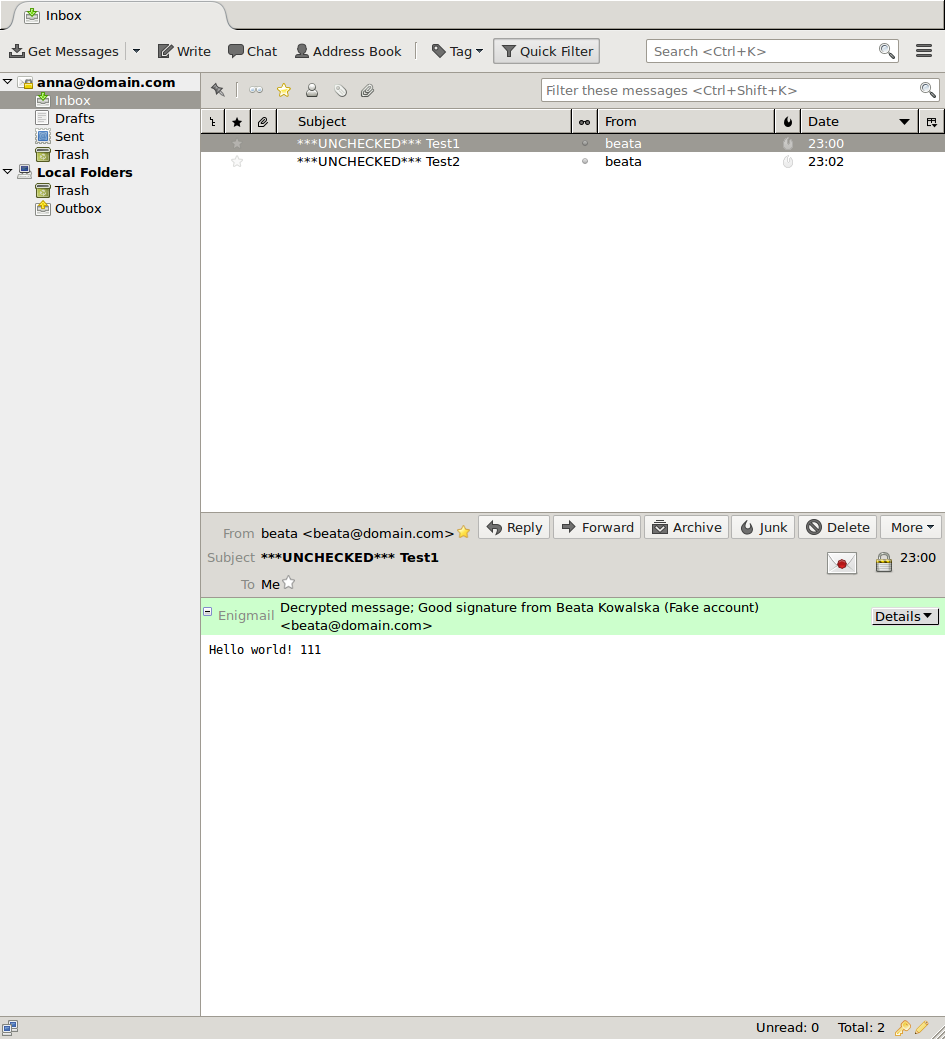
\includegraphics[width=0.9\textwidth]{images/ok.png}
    \label{fig:ok}
    \caption{Message from user whose key was signed by admin viewed in Thunderbird.}
\end{figure}

Then to test if the key validation works properly, we generated another key pair and
sent it to the key server, but without it being signed by admin. Then we sent an email
and signed it with the new key. As shown on figure \ref{fig:nonrepudiation-fail},
the Thunderbird on the receiving end was unable to verify the signature and warned
the recipient of this fact by saying the key is \code{UNTRUSTED}.

\begin{figure}[H]
\centering
    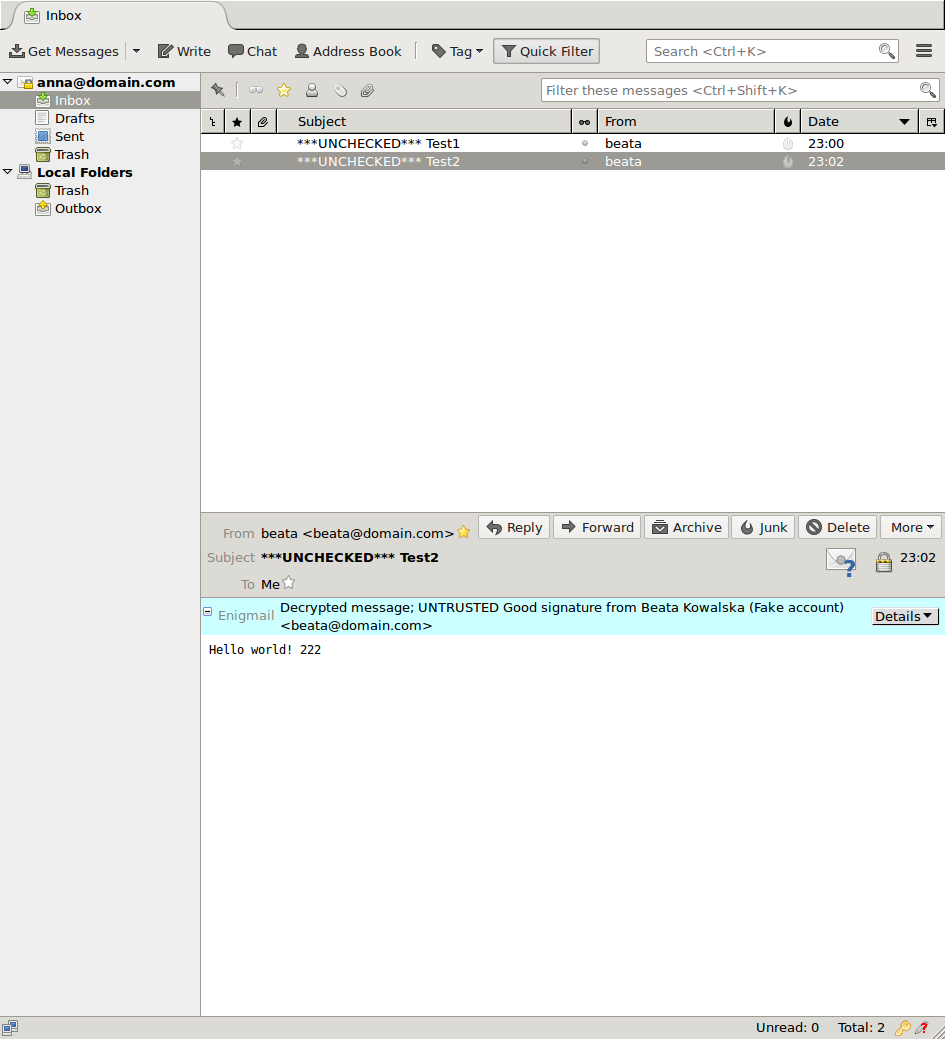
\includegraphics[width=0.9\textwidth]{images/nonrepudiation-fail.png}
    \label{fig:nonrepudiation-fail}
    \caption{Message from user whose key is not signed by admin viewed in Thunderbird.}
\end{figure}

Then we tested the encryption capabilities. We deleted beata's private key and then sent
a mail to her. Beata's thunderbird found it impossible to decrypt the message and
reported error. This shows that it is impossible to read a message without having the
required private key, which should include only the intended recipient.

\begin{figure}[H]
\centering
    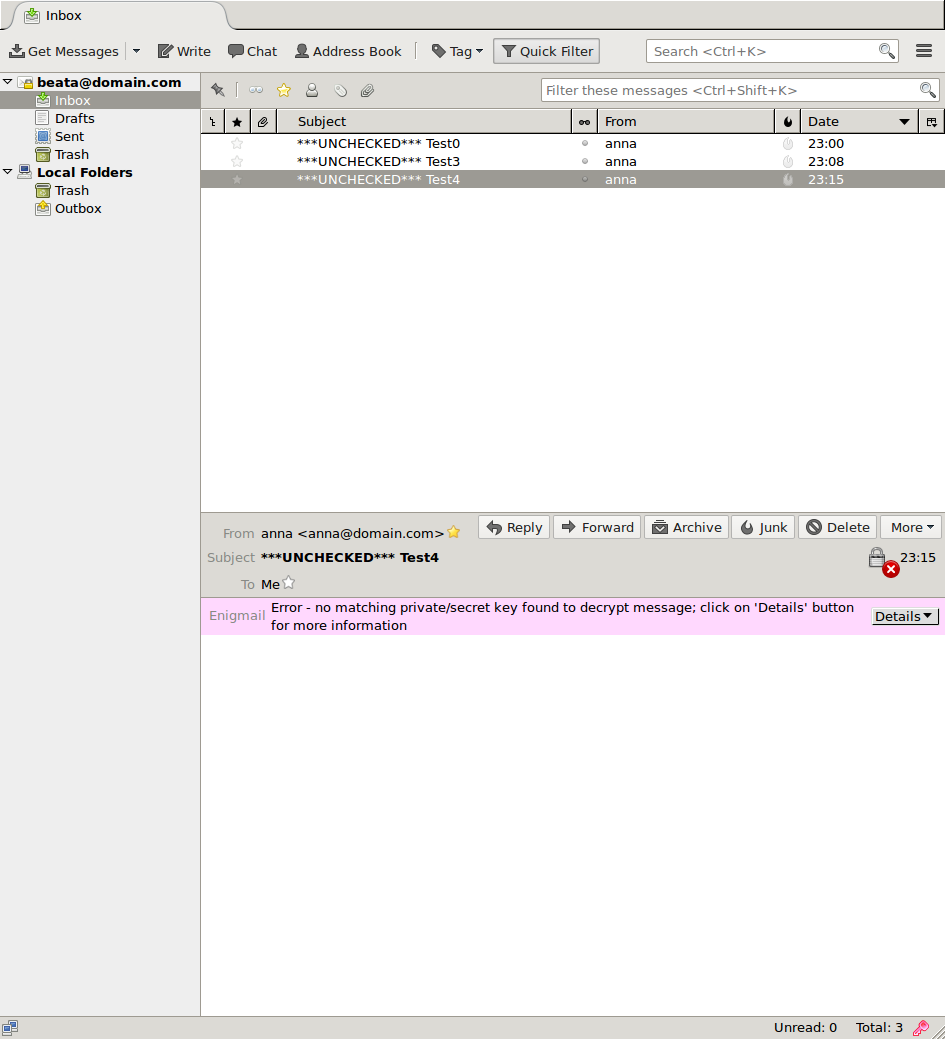
\includegraphics[width=0.9\textwidth]{images/confidentiality-fail.png}
    \label{fig:confidentiality-fail}
    \caption{An encrypted message addressed to a different user viewed in Thunderbird.}
\end{figure}

\section{Discussion}

PGP is widely considered to be secure and we have confirmed in the previous section that
we have set up it correctly. We can thus claim that we have achieved a secure transfer
of files.

After initial setup of GPG we integrated it with Thunderbird via Enigmail plugin. As
a result sending secure emails became almost as easy as sending normal ones and
this level of ease of use is nowadays acceptable to a majority of people. We have
therefore reached the goal of the practical workshop.

\begin{thebibliography}{0}
    \bibitem{paranoid} Michael W. Lucas, PGP \& GPGEmail for the Practical Paranoid
    \bibitem{documentation} Using the GNU Privacy Guard, \url{https://www.gnupg.org/documentation/manuals/gnupg.pdf}
\end{thebibliography}

\end{document}
